\documentclass{ximera}

\newcommand{\dfn}{\textbf}
\renewcommand{\vec}[1]{{\overset{\boldsymbol{\rightharpoonup}}{\mathbf{#1}}}\hspace{0in}}
%% Simple horiz vectors
\renewcommand{\vector}[1]{\left\langle #1\right\rangle}
\newcommand{\arrowvec}[1]{{\overset{\rightharpoonup}{#1}}}
\newcommand{\R}{\mathbb{R}}
\newcommand{\transpose}{\intercal}
\newcommand{\ro}{\texttt{R}}%% row operation
\newcommand{\dotp}{\bullet}%% dot product

\usetikzlibrary{calc,bending}
\tikzset{>=stealth}


\usepackage{mdframed} % For framing content
%\usepackage{ifthen}   % For conditional statements

% Define the 'concept' environment with an optional header
\newenvironment{concept}[1][]{%
  \begin{mdframed}[linecolor=black, linewidth=2pt, innertopmargin=5pt, innerbottommargin=5pt, skipabove=12pt, skipbelow=12pt]%
    \noindent\large\textbf{#1}\normalsize%
}{%
  \end{mdframed}%
}











%% \colorlet{textColor}{black}
%% \colorlet{background}{white}
%% \colorlet{penColor}{blue!50!black} % Color of a curve in a plot
%% \colorlet{penColor2}{red!50!black}% Color of a curve in a plot
%% \colorlet{penColor3}{red!50!blue} % Color of a curve in a plot
%% \colorlet{penColor4}{green!50!black} % Color of a curve in a plot
%% \colorlet{penColor5}{orange!80!black} % Color of a curve in a plot
%% \colorlet{penColor6}{yellow!70!black} % Color of a curve in a plot
%% \colorlet{fill1}{penColor!20} % Color of fill in a plot
%% \colorlet{fill2}{penColor2!20} % Color of fill in a plot
%% \colorlet{fillp}{fill1} % Color of positive area
%% \colorlet{filln}{penColor2!20} % Color of negative area
%% \colorlet{fill3}{penColor3!20} % Fill
%% \colorlet{fill4}{penColor4!20} % Fill
%% \colorlet{fill5}{penColor5!20} % Fill
%% \colorlet{gridColor}{gray!50} % Color of grid in a plot


\author{Parisa Fatheddin \and Tae Eun Kim \and Bart Snapp}


%% https://ghenshaw-work.medium.com/3-ways-to-understand-matrix-multiplication-fe8a007d7b26


\title{Matrices, products, and equations}


\begin{document}
\begin{abstract}
  A concrete introduction to matrices and their connections to systems
  of equations.
\end{abstract}
\maketitle

\begin{quote}
  Probably no other area of mathematics has been applied in such
  numerous and diverse contexts as the theory of matrices. In
  mechanics, electromagnetics, statistics, economics, operations
  research, the social sciences, and so on, the list of applications
  seems endless. By and large this is due to the utility of matrix
  structure and methodology in conceptualizing sometimes complicated
  relationships and in the orderly processing of otherwise tedious
  algebraic calculations and numerical manipulations.



  \hfill ---\link[J.\ Cochran]{https://go.osu.edu/cochran}
\end{quote}



A \dfn{matrix} is simply a rectangular array of numbers
\[
  A =
  % \underset{\displaystyle\boldsymbol{5}~\textbf{columns}}{
  \underset{\raisebox{-2ex}{\text{\bf 5 columns}}}{
    \begin{pmatrix}
      a_{1,1} & a_{1,2} & a_{1,3} & a_{1,4} & a_{1,5} \\
      a_{2,1} & a_{2,2} & a_{2,3} & a_{2,4} & a_{2,5} \\
      a_{3,1} & a_{3,2} & a_{3,3} & a_{3,4} & a_{3,5} \\
      a_{4,1} & a_{4,2} & a_{4,3} & a_{4,4} & a_{4,5}
    \end{pmatrix}}
  \quad\text{\bf 4 rows}
\]
We give the \dfn{dimensions of a matrix} by stating its number of rows
and number of columns. The number of rows comes first and the number
of columns second, so $A$ above is a $(4\times 5)$-matrix.
\begin{question}
  Which of the following matrices are $3\times 2$ matrices?
  \begin{selectAll}
    \pdfOnly{\begin{multicols}{4}}
      \choice{$\begin{pmatrix}
        2 & 4 & 8\\
        5 & 9 & -1\\
        6 & 0 & 1
      \end{pmatrix}$}
    \choice{$\begin{pmatrix}
      0 & 1 &3\\
      0 & 0 & 2
    \end{pmatrix}$}
  \choice[correct]{$\begin{pmatrix}
    2 & 1 \\
    4 & 5 \\
    -1 & 0
  \end{pmatrix}$}
\choice[correct]{$\begin{pmatrix}
  0 & 0\\
  0 & 0 \\
  0 & 0
\end{pmatrix}$}
\pdfOnly{\end{multicols}}
\end{selectAll}
\end{question}


% We can use similar notation to talk about specific entries of a
% matrix. Above, $a_{i,j}$ is the \dfn{$\boldsymbol{(i,j)}$-entry} of
% the matrix $M$ (we usually use capital letters for matrices). Often
% people write $M_{i,j}$ (or just $M_{ij}$) to mean the $(i,j)$-entry of
% the matrix $M$.

%% TK: For now, I am using the concept environment. Not sure whether
%% to style this differently by introducing a new environment.
\begin{concept}[Notation.]
  Scalars, vectors, and matrices are the key players in the land of
  linear algebra. Now that they are all introduced, here are our
  notational convention for the remainder of the textbook.

  We generally use
  \begin{itemize}
  \item upper-case regular type (e.g., $A, B, C, \ldots$) for matrices;
  \item lower-case bold type (e.g., $\vec{u}, \vec{v}, \vec{w}, \ldots$)
    for vectors;
  \item lower-case regular type (e.g., $a, b, c, \ldots$) for scalars.
  \end{itemize}

  When it comes to vectors, we learned various ways to express them in
  the previous chapter, but we will stick with one of them:

  \begin{center}
    Unless otherwise specified, vectors are column vectors by default.
  \end{center}

  This is a widely used convention across many fields of STEM due to
  practical and theoretical reasons. We will indicate a row vector by
  explicitly transposing a column vector. For typesetting convenience,
  the components of a column vector are often displayed by transposing
  the corresponding column vector as in
  \[
    \vec{v} =
    \begin{pmatrix}
      4 & 3 & 2 & 1 & 0
    \end{pmatrix}^\transpose
    \quad\text{or}\quad
    \vec{v}^\transpose =
    \begin{pmatrix}
      4 & 3 & 2 & 1 & 0
    \end{pmatrix}.
  \]

  Component indices are denoted by subscripts, usually $i$ through
  $n$. For example, the $i$th entry of a vector $\vec{v}$ is denoted
  by $v_i$. % or $\left[ \vec{v} \right]_i$.
  %% TK: How about this?
  The $(i,j)$-entry of a matrix $A$ is denoted by $a_{i,j}$,
  $a_{ij}$ or even $A_{i,j}$.
  % $\left[ A \right]_{ij}$.
\end{concept}


\begin{question}
  If
  \[A= \begin{pmatrix}
    -3 & 0 & 1\\
    4 & 5 & -2\\
    0 & 9 & -1
  \end{pmatrix}
\]
what are the entries $a_{1,2}$, $a_{2,2}$, $a_{3,2}$?
\begin{prompt}
  \[
    a_{1,2} = \answer{0}, \quad a_{2,2} = \answer{5}, \quad a_{3,2} = \answer{9}
  \]
\end{prompt}
\end{question}

Next we'll discuss how matrices arise in different contexts.


\section{Matrices store data}


A matrix can be thought of as a ``mathematical spreadsheet.'' With a
spreadsheet you have rows and columns of data.  The data we're
typically interested in comes in the form of vectors.  You can think
of a matrix as vectors stacked together either horizontally or
vertically.

\begin{example}[Population Counts] %https://worldpopulationreview.com/states/states-by-race
  In a previous example, we encoded the $2023$
  \link[demographics]{https://worldpopulationreview.com/states/states-by-race}~of
  the twelve Midwestern States as $6$-dimensional vectors represented
  as ordered tuples. Represent this data by a $12\times 6$
  matrix. Explain what the entry at position $(7,5)$ represents.
  \begin{explanation}
    Since ordered-tuples are \wordChoice{\choice[correct]{horizontal}\choice{vertical}} it makes sense to
    concatenate this data by stacking it horizontally into a matrix:
    \[
      \begin{pmatrix}
        \vec{p}_{\texttt{IA}} \\
        \vec{p}_{\texttt{IL}} \\
        \vec{p}_{\texttt{IN}} \\
        \vec{p}_{\texttt{KA}} \\
        \vec{p}_{\texttt{MI}} \\
        \vec{p}_{\texttt{MN}} \\
        \vec{p}_{\texttt{MO}} \\
        \vec{p}_{\texttt{ND}} \\
        \vec{p}_{\texttt{NE}} \\
        \vec{p}_{\texttt{OH}} \\
        \vec{p}_{\texttt{SD}} \\
        \vec{p}_{\texttt{WI}}
      \end{pmatrix}
      =
      \begin{pmatrix}
        2806418 & 117035 & 10538 & 79296 & 3941 & 132783\\
        8874067 & 1796660 & 33972 & 709567 & 5196 & 1296702\\
        5510354 & 631923 & 14030 & 158705 & 2205 & 379676\\
        2416165 & 165837 & 22278 & 87093 & 2344 & 218902\\
        7735902 & 1360149 & 50035 & 316844 & 3117 & 507860\\
        4572149 & 359817 & 54558 & 275242 & 2201 & 336199\\
        4978046 & 698043 & 24274 & 123810 & 8887 & 291100\\
        651470 & 23959 & 39165 & 11979 & 1004 & 32817\\
        1641256 & 91896 & 16875 & 47944 & 1235 & 124620\\
        9394878 & 1442655 & 20442 & 268527 & 3907 & 544866\\
        735228 & 18836 & 74975 & 12413 & 544 & 37340\\
        4895065 & 367889 & 48674 & 163396 & 2672 & 329279
      \end{pmatrix}
    \]
    Note that the above is a $\answer[given]{12}\times \answer[given]{6}$ matrix. The $(7, 5)$-entry is
    $\answer[given]{8887}$ which is the number of Hawaiians in Missouri (MO).
  \end{explanation}
\end{example}





\begin{example}[Grayscale Image]
  Here is a very low resolution grayscale image of the number $6$:
  \begin{center}
    \newcommand{\matrixData}{{
        {0, 0.01, 0, 0, 0, 0, 0},
        {0, 0, 0.06, 0.18, 0.18, 0.01, 0},
        {0, 0.38, 0.64, 0.21, 0.37, 0.79, 0.06},
        {0.12, 0.99, 0.12, 0.01, 0, 0.11, 0.02},
        {0.34, 0.94, 0.32, 0.41, 0.64, 0.55, 0.02},
        {0.35, 0.97, 0.09, 0, 0.05, 0.98, 0.43},
        {0.14, 0.98, 0.13, 0, 0.01, 0.94, 0.39},
        {0, 0.34, 0.56, 0.29, 0.47, 0.51, 0.01},
        {0, 0, 0, 0.07, 0.03, 0, 0},
        {0, 0.01, 0, 0, 0, 0.02, 0}
      }}
    \begin{tikzpicture}[scale=.5]
      \foreach \y in {1, ..., 8} {
        \foreach \x in {0, 1, ..., 6} {
          \pgfmathsetmacro\val{\matrixData[\y][\x]}
          \fill[black, opacity=\val] (\x, -\y) rectangle (\x+1, -\y-1);
          \draw (\x, -\y) rectangle (\x+1, -\y-1);
        }
      }
    \end{tikzpicture}
  \end{center}
  We can represent this data as an $8\times 7$ matrix where $0$
  represents ``black,'' $1$ represents ``white,'' and numbers in between represent ``shades of gray.''
  \[
    \begin{pmatrix}
      1 & 1 & 0.94 & 0.82 & 0.82 & 0.99 & 1 \\
      1 & 0.62 & 0.36 & 0.79 & 0.63 & 0.21 & 0.94 \\
      0.88 & 0.01 & 0.88 & 0.99 & 1 & 0.89 & 0.98 \\
      0.66 & 0.06 & 0.68 & 0.59 & 0.36 & 0.45 & 0.98 \\
      0.65 & 0.03 & 0.91 & 1 & 0.95 & 0.02 & 0.57 \\
      0.86 & 0.02 & 0.87 & 1 & 0.99 & 0.06 & 0.61 \\
      1 & 0.66 & 0.44 & 0.71 & 0.53 & 0.49 & 0.99 \\
      1 & 1 & 1 & 0.93 & 0.97 & 1 & 1 \\
    \end{pmatrix}
  \]
  Interpret the meaning of the $(4,6)$-entry of the matrix.
  \begin{explanation}
    Here the $(4,6)$-entry of the matrix is
    $\answer[given]{0.71}$. This represents a shade of gray that is
    closer to \wordChoice{\choice[correct]{white}\choice{black}} than
    it is to  \wordChoice{\choice{white}\choice[correct]{black}}.
  \end{explanation}
\end{example}




\begin{example}[Consumer Data]
  The \textit{MOOCulus Streaming Service} wasn't always as popular as
  it is today. When it started there were only $5$ subscribers who
  happen to be our friends, and only $3$ movies are streamed:
  \textit{Time Bandits}, \textit{Brazil} and \textit{The Adventures of Baron
    Munchausen}. For simplicity and privacy reasons, we call the
  subscribers $\vec c_1$, $\vec c_2$, $\vec c_3$, $\vec c_4$, and
  $\vec c_5$ and movies will coorespond to the first, second and third
  entries of the vectors $\vec v_i$:
  \begin{align*}
    \vec v_{1}^\transpose &= \begin{pmatrix}0 & 1 & 2\end{pmatrix}\\
    \vec v_{2}^\transpose &= \begin{pmatrix}1 & 0 & 1\end{pmatrix}\\
    \vec v_{3}^\transpose &= \begin{pmatrix}3 & 1 & 0\end{pmatrix}\\
    \vec v_{4}^\transpose &= \begin{pmatrix}1 & 0 & 0\end{pmatrix}\\
    \vec v_{5}^\transpose &= \begin{pmatrix}0 & 6 & 0\end{pmatrix}
  \end{align*}
  Here, for each vector, the first value is the number of times the
  consumer watched \textit{Time Bandits}, the second value is the
  number of times the consumer watched \textit{Brazil}, and the third
  value is the number of times the consumer watched \textit{The
    Adventures of Baron Munchausen}.  This data can be packaged into a
  $5 \times 3$ matrix $M$:
  \[
    M =
    \begin{pmatrix}
      0 & 1 & 2\\
      1 & 0 & 1\\
      3 & 1 & 0\\
      1 & 0 & 0\\
      0 & 6 & 0
    \end{pmatrix}.
  \]
  \begin{itemize}
  \item Compute the sum of the entries in the third row and interpret the result in this context.
  \item Compute the sum of the entries in the second column and interpret the result in this context.
  \end{itemize}
  \begin{explanation}
    The sum across the third row is $\answer[given]{4}$. This means
    that consumer $\vec{c}_{\answer[given]{3}}$ streamed a total of  $\answer[given]{4}$ \wordChoice{\choice{distinct}\choice[correct]{possibly nondistinct}} movies.


    On the other hand, the sum along the second column is $\answer[given]{8}$. This
    means that \wordChoice{\choice{Time Bandits}\choice[correct]{Brazil}\choice{The Adventures of Baron Munchausen}} has been watched $\answer[given]{8}$ times.
  \end{explanation}
\end{example}





\section{Multiplying matrices and vectors}

% %% TK suggestion %%%%%%%%%%%%%%%%%%%%%%%%%%%%%%%%%%%%%%%%%%%%%%%%%%%%%%%%%%%%%%
%% Below is inspired, among many others, by Golub and van Loan. They
%% call it a ``row/column partitioning'' of a matrix. In the numerical
%% linear algebra community, they use M(i,:), M(:,j) for your row_i(M)
%% and col_j(M), respectively.

% \hrulefill

% Let $A$ be an $m \times n$ matrix
% \[
%   A =
%   \begin{pmatrix}
%     a_{11} & a_{12} & \cdots & a_{1n} \\
%     a_{21} & a_{22} & \cdots & a_{2n} \\
%     \vdots & \vdots & \ddots & \vdots \\
%     a_{m1} & a_{m2} & \cdots & a_{mn}
%   \end{pmatrix}.
% \]
% Instead of thinking of or expressing $A$ in terms of its components as
% above, we can think at the level of vectors. That is, $A$ can be
% viewed as a concatenation of $n$ column vectors
% \[
%   A =
%   \begin{pmatrix}
%     \vec{a}_1 & \vec{a}_2 & \cdots & \vec{a}_n
%   \end{pmatrix},\quad\text{where}\quad
%   \vec{a}_1 =
%   \begin{pmatrix}
%     a_{11} \\ a_{21} \\ \vdots \\ a_{m1}
%   \end{pmatrix},\,
%   \vec{a}_2 =
%   \begin{pmatrix}
%     a_{12} \\ a_{22} \\ \vdots \\ a_{m2}
%   \end{pmatrix},\,\cdots,\,
%   \vec{a}_n =
%   \begin{pmatrix}
%     a_{1n} \\ a_{2n} \\ \vdots \\ a_{mn}
%   \end{pmatrix};
% \]
% or as a stack of $m$ row vectors
% \[
%   A =
%   \begin{pmatrix}
%     \vec{\boldsymbol \alpha}_1^\transpose \\
%     \vec{\boldsymbol \alpha}_2^\transpose \\
%     \vdots \\
%     \vec{\boldsymbol \alpha}_m^\transpose
%   \end{pmatrix},\quad\text{where}\quad
%   \vec{\boldsymbol \alpha}_1 =
%   \begin{pmatrix}
%     a_{11} \\ a_{12} \\ \vdots \\ a_{1n}
%   \end{pmatrix},\,
%   \vec{\boldsymbol \alpha}_2 =
%   \begin{pmatrix}
%     a_{21} \\ a_{22} \\ \vdots \\ a_{2n}
%   \end{pmatrix},\,\cdots,\,
%   \vec{\boldsymbol \alpha}_m =
%   \begin{pmatrix}
%     a_{m1} \\ a_{m2} \\ \vdots \\ a_{mn}
%   \end{pmatrix}.
% \]
% With this vector-level perspective, we can develop a meaningful way to
% multiply matrices and vectors based on the dot product.

% Recall that the dot product of two vectors is given by
% \begin{align*}
%   \vec{a} \dotp \vec{b} & = a_1b_1 + a_2b_2 +\dots+a_nb_n.
% \end{align*}

% \subsection{Multiplying a matrix by a column vector}
% Let $A$ be an $m \times n$ matrix and $\vec{x}$ be an $n$-vector. Then the
% product $A \vec{x}$ is an allowed operation producing a column
% $m$-vector given by
% \[
%   A \vec{x} =
%   \begin{pmatrix}
%     \vec{\boldsymbol \alpha}_1^\transpose \\
%     \vec{\boldsymbol \alpha}_2^\transpose \\
%     \vdots \\
%     \vec{\boldsymbol \alpha}_m^\transpose
%   \end{pmatrix} \vec{x}
%   =
%   \begin{pmatrix}
%     \vec{\boldsymbol \alpha}_1 \dotp \vec{x} \\
%     \vec{\boldsymbol \alpha}_2 \dotp \vec{x} \\
%     \vdots \\
%     \vec{\boldsymbol \alpha}_m \dotp \vec{x}
%   \end{pmatrix}.
% \]
% The product can also be viewed as
% \[
%   A \vec{x} =
%   \begin{pmatrix}
%     \vec{a}_1 & \vec{a}_2 & \cdots & \vec{a}_n
%   \end{pmatrix}
%   \begin{pmatrix}
%     x_1 \\ x_2 \\ \vdots \\ x_n
%   \end{pmatrix}
%   = \vec{a}_1 x_1 + \vec{a}_2 x_2 + \cdots + \vec{a}_n x_n.
% \]

% \subsection{Multiplying a row vector by a matrix}
% Let $A$ be an $m \times n$ matrix and $\vec{y}$ be an $m$-vector. Then the
% product $\vec{y}^\transpose A$ is an allowed operation producing a row
% $n$-vector given by
% \[
%   \vec{y}^\transpose A =
%   \vec{y}^\transpose
%   \begin{pmatrix}
%     \vec{a}_1 & \vec{a}_2 & \cdots & \vec{a}_n
%   \end{pmatrix}
%   =
%   \begin{pmatrix}[c|c|c|c]
%     \vec{y}^\transpose \dotp \vec{a}_1
%     & \vec{y}^\transpose \dotp \vec{a}_2
%     & \cdots
%     & \vec{y}^\transpose \dotp \vec{a}_n
%   \end{pmatrix}.
% \]
% Alternately, the product can be viewed as
% \[
%   \vec{y}^\transpose A =
%   \begin{pmatrix}
%     y_1 & y_2 & \cdots & y_m
%   \end{pmatrix}
%   \begin{pmatrix}
%     \vec{\boldsymbol \alpha}_1^\transpose \\
%     \vec{\boldsymbol \alpha}_2^\transpose \\
%     \vdots \\
%     \vec{\boldsymbol \alpha}_m^\transpose
%   \end{pmatrix}
%   = y_1 \vec{\boldsymbol \alpha}_1^\transpose
%   + y_2 \vec{\boldsymbol \alpha}_2^\transpose
%   + \cdots
%   + y_m \vec{\boldsymbol \alpha}_m^\transpose.
% \]
% \hrulefill
% %% End of TK suggestion %%%%%%%%%%%%%%%%%%%%%%%%%%%%%%%%%%%%%%%%%%%%%%%%%

We can define a meaningful way to multiply matrices and vectors based
on the dot product. Recall that the dot product of two vectors is
given by
\begin{align*}
  \begin{pmatrix}
    a_1\\
    a_2\\
    \vdots\\
    a_n
  \end{pmatrix}
  \dotp
  \begin{pmatrix}
    b_1\\
    b_2\\
    \vdots\\
    b_n
  \end{pmatrix}
  &=\begin{pmatrix} a_1 & a_2 & \cdots & a_n\end{pmatrix}\dotp\begin{pmatrix} b_1 & b_2 & \cdots & b_n\end{pmatrix}\\
  &= \sum_{i=1}^n a_ib_i\\
  & = a_1b_1 + a_2b_2 +\dots+a_nb_n.
\end{align*}
We can extend this idea to multiplying matrices by vectors and to
multiplying vectors by matrices.

\subsection{Multiplying a matrix by a column vector}
% Given an $m\times n$ matrix $M$ and an $n$-vector $\vec{a}$, \textbf{the
%   number of columns of the matrix equals the number of entries of
%   the vector} and we can compute the product $M\vec{a}$, defining
Let $M$ be an $m\times n$ matrix and $\vec{a}$ be a column $n$-vector. In
this case, \textbf{the number of columns of the matrix equals the
  number of entries of the vector}, and the product $M\vec{a}$ is
defined by
\[
  M \vec{a} =
  \begin{pmatrix}
    \row_1(M)^\transpose \dotp \vec{a} \\
    \row_2(M)^\transpose \dotp \vec{a} \\
    \vdots \\
    \row_m(M)^\transpose \dotp \vec{a}
  \end{pmatrix},
\]
where $\row_i(M)$ represents the $i$th row of $M$. Note that
$M\vec{a}$ is a column $m$-vector. Below schematically depicts the
nature of the matrix-vector product:
\[
  \begin{matrix}
    \begin{pmatrix}
      \bullet & \bullet & \bullet & \bullet & \bullet \\
      \bullet & \bullet & \bullet & \bullet & \bullet \\
      \bullet & \bullet & \bullet & \bullet & \bullet \\
    \end{pmatrix}
    &
      \begin{pmatrix}
        \bullet \\ \bullet \\ \bullet \\ \bullet \\ \bullet
      \end{pmatrix}
    & = &
          \begin{pmatrix}
            \bullet \\ \bullet \\ \bullet
          \end{pmatrix}
    \\
    \begin{pmatrix}
      m\times n\\
      \text{matrix}
    \end{pmatrix}
    &
      \begin{pmatrix}
        n\text{-vector}\\
        \text{column}
      \end{pmatrix}
    & &
        \begin{pmatrix}
          m\text{-vector}\\
          \text{column}
        \end{pmatrix}
  \end{matrix}
\]




\subsection{Multiplying a row vector by a matrix}
% If on the other hand, $M$ is still a $m\times n$ matrix, but now
% $\vec{b}$ is an $m$-vector expressed as a row, \textbf{the number of
%   entries of the vector must equal the number of rows of the matrix}
% and we can compute the product $\vec{b}M$, defining
If, on the other hand, $M$ is still an $m\times n$ matrix, but now
$\vec{b}$ is a row $m$-vector, \textbf{the number of entries of the
  vector equals the number of rows of the matrix}, and the product
$\vec{b} M$ is defined by
\[
  \vec{b} M =
  \begin{pmatrix}
    \vec{b}\dotp \col_1(M)^\transpose &
    \vec{b}\dotp \col_2(M)^\transpose &
    \cdots &
    \vec{b}\dotp \col_n(M)^\transpose
  \end{pmatrix},
\]
where $\col_i(M)$ represents the $i$th column of $M$. Note that
$\vec{b} M$ is a row $n$-vector. Below is a schematic of
the vector-matrix product:
\[
  \begin{matrix}
    \begin{pmatrix}
      \bullet & \bullet & \bullet
    \end{pmatrix}
    &
      \begin{pmatrix}
        \bullet & \bullet & \bullet & \bullet & \bullet \\
        \bullet & \bullet & \bullet & \bullet & \bullet \\
        \bullet & \bullet & \bullet & \bullet & \bullet
      \end{pmatrix}
    &
      =
    &
      \begin{pmatrix}
        \bullet & \bullet & \bullet & \bullet & \bullet
      \end{pmatrix}
    \\
    \begin{pmatrix}
      m\text{-vector}\\
      \text{row}
    \end{pmatrix}
    &
      \begin{pmatrix}
        m\times n\\
        \text{matrix}
      \end{pmatrix}
    & &
        \begin{pmatrix}
          n\text{-vector}\\
          \text{row}
        \end{pmatrix}
  \end{matrix}
\]


\begin{question}
  Let
  \[
    A=\begin{pmatrix}
      2 & 0 & -1\\
      5 & 1 & -2\\
      1 & 0 & 4
    \end{pmatrix}
    \quad\text{and}\quad
    \vec{v} = \begin{pmatrix}
      1\\
      0\\
      2
    \end{pmatrix}.
  \]
  Compute the following, if possible.
  \begin{prompt} Write ``NA'' for each entry if the multiplication is not possible.\end{prompt}
  \begin{enumerate}
    \pdfOnly{\begin{multicols}{4}}
    \item $\vec{v} A$
      \begin{prompt}
        \[
          =\begin{pmatrix}
            \answer[given,format=string]{NA}\\
            \answer[given,format=string]{NA}\\
            \answer[given,format=string]{NA}
          \end{pmatrix}
        \]
      \end{prompt}
    \item $A\vec{v}$
      \begin{prompt}
        \[
          = \begin{pmatrix}
            \answer[given]{0}\\
            \answer[given]{-4}\\
            \answer[given]{9}
          \end{pmatrix}
        \]
      \end{prompt}
    \item $\vec{v}^{\transpose} A$
      \begin{prompt}
        \[
          = \begin{pmatrix}
            \answer[given]{2} & \answer[given]{0} & \answer[given]{7}
          \end{pmatrix}
        \]
      \end{prompt}
    \item $A\vec{v}^{\transpose}$
      \begin{prompt}
        \[
          = \begin{pmatrix}
            \answer[given,format= string]{NA} & \answer[given,format= string]{NA} & \answer[given,format= string]{NA}
          \end{pmatrix}
        \]
      \end{prompt}
    \pdfOnly{\end{multicols}}
  \end{enumerate}
\end{question}

Our next proposition relates the transpose and the dot product.
%% Note, if $A$ and $B$ are matrices, $\vec{x}$ and $\vec{y}$ are
%% vectors, and one \textit{resonably} writes
%% \[
%%   \vec x A\quad\text{or}\quad  B \vec y
%% \]
%% then $\vec{x}$ is necessarially a row vector and $\vec{y}$ is necessarially a column vector. This is related to our next proposition:


\begin{proposition}[Dot product and transpose]
  Given $n$-vectors, $\vec{x}$ and $\vec y$ with
  \begin{itemize}
  \item $\vec{x}$ expressed as a row,
  \item $\vec{y}$ expressed as a column,
  \end{itemize}
  then
  \[
    \vec{x}^\transpose\dotp \vec{y} = \vec{x}\dotp\vec{y}^\transpose.
  \]

  %% TK: Rephrased this.  Question: Should we maybe put this after
  %% introducing matrix product?
  %% BS: We just did matrix*vector and vector*matrix... I kinda like it here.
  \begin{explanation}
    In this case, interpret $\vec{x}$ as a $1\times n$ matrix, and
    $\vec{y}$ as a column vector. By our definition above
    \[
      \vec{x}\vec{y} = \vec{x}^\transpose\dotp \vec{y}.
    \]
    If we interpret $\vec{x}$ as a row vector, and
    $\vec{y}$ as a $n\times 1$ matrix, by our definition above
    \[
      \vec{x}\vec{y} = \vec{x}\dotp\vec{y}^\transpose.
    \]
    Hence
    \[
      \vec{x}^\transpose\dotp \vec{y} = \underset{\begin{matrix}\text{matrix}\\\text{product}\end{matrix}}{\vec{x}\vec{y}} = \vec{x}\dotp\vec{y}^\transpose.
    \]
    %% Note that the matrix product $\vec{x} \vec{y}$ makes sense because
    %% the number of columns of the first matrix $\vec{x}$ equals the
    %% number of rows of the second matrix $\vec{y}$.
    % hence they are equal.
  \end{explanation}
\end{proposition}


\begin{example}[Grayscale Image]%% https://commons.wikimedia.org/wiki/File:Cat_face_closeup.jpg
  Here is a grayscale image of a cat:
  \begin{image}
    
\includegraphics[width=.5\textwidth]{catfaceGS.jpg}
  \end{image}
  This image has a resolution of $600$ rows by $800$ columns. With a
  whopping $480000$ entries, the matrix representing this image is too
  large to conveniently express, so let's just call it $C$, for
  \textit{cat}; or perhaps \textit{convenient}.  Explain how to
  express $c_{ij}$ as a product of $C$ and vectors of the forms:
  \begin{itemize}
  \item A $600$-vector expressed as a row
    \[
      \vec r_i^\transpose =
      \underbrace{
        \begin{pmatrix} 0 & \cdots  & 0 & 1 & 0 & \cdots & 0 \end{pmatrix}
      }_{
        \begin{matrix}
          \displaystyle \text{all entries are zero} \\
          \displaystyle \text{ except for the $i$th}
        \end{matrix}
      }
    \]
  \item A $800$-vector expressed as a column
    \[
      \vec c_j = \left.
        \begin{pmatrix} 0 \\ \vdots  \\ 0 \\ 1 \\ 0 \\ \vdots \\ 0 \end{pmatrix}
        \quad
      \right\}
      \quad
      \begin{matrix}
        \text{all entries are zero}\\
        \text{except for the $j$th}
      \end{matrix}
    \]
  \end{itemize}
  \begin{explanation}
    First note that $\vec r_i^\transpose C$ computes the $i$th
    \wordChoice{\choice[correct]{row}\choice{column}} of the matrix
    $C$. On the other hand, $(\vec r_i^\transpose C)\vec c_j$ computes the $j$th
    \wordChoice{\choice{row}\choice[correct]{column}} of the matrix
    $\vec r_i^\transpose C$. Hence
    \[
      \vec r_i^\transpose C \vec{c}_j
    \]
    computes $c_{ij}$. In other words, the operation
    $\vec{r}_i^\transpose C \vec{c}_j$ extracts the grayscale information of the
    pixel on the $i$th row and the $j$th column of the image.
  \end{explanation}
\end{example}


The grayscale image example above showcases a utility of matrix-vector
product in extracting a row or a column of a given matrix.



%% TK: This may be a good place to introduce this theme. We may
%% revisit later, e.g., after matrix-matrix product or when discussing
%% row-operations.
%% \begin{concept}[Row and Column Actions]
%%   The grayscale image example above showcases a utility of
%%   matrix-vector product in extracting a row or a column of a given
%%   matrix. It turns out that matrix-vector products can emulate
%%   various operations on rows or columns of a matrix that are more
%%   involved than simple extraction.

%%   The general theme is as follows. Let $M$ be an $m \times n$ matrix,
%%   $\vec{r}$ a $1 \times m$ row vector, and $\vec{c}$ an $n \times 1$ column
%%   vector. Then
%%   \begin{description}
%%   \item[Row operation.] The vector-matrix product $\vec{r} M$ emulates an operation
%%     on rows of $M$. The components of $\vec{r}$ conveys the
%%     information about the row operation.
%%   \item[Column operation.] The matrix-vector product $M \vec{c}$
%%     emulates an operation on columns of $M$. The components of
%%     $\vec{c}$ conveys the information about the column operation.
%%   \end{description}
%%   This is an important theme in linear algebra.
%% \end{concept}


\section{Systems of equations}



One important use of matrices is to solve systems of equations. By matrix multiplication, one can check that
\begin{eqnarray*}
  4x+2y+z &=& 5\\
  2x+3y &=& 6\\
  5y -z &=& 8
\end{eqnarray*}
can be written as
\[
  \begin{pmatrix}
    4 & 2 & 1 \\
    2 & 3 & 0\\
    0 & 5 & -1
  \end{pmatrix}
  \begin{pmatrix}
    x \\
    y\\
    z
  \end{pmatrix}
  = \begin{pmatrix}
    5 \\
    6\\
    8
  \end{pmatrix}
\]
as multiplying the left-hand side above we have
\[
  \begin{pmatrix}
    4x+2y+z\\
    2x+3y\\
    5y-z
  \end{pmatrix} = \begin{pmatrix}
    5\\
    6\\
    8
  \end{pmatrix}.
\]
With this in mind, it is common to write
\[
  A = \begin{pmatrix}
    4 & 2 & 1 \\
    2 & 3 & 0\\
    0 & 5 & -1
  \end{pmatrix},\quad\vec x = \begin{pmatrix} x \\ y \\ z\end{pmatrix},
  \quad\vec b = \begin{pmatrix} 5 \\6\\8\end{pmatrix},
\]
allowing us to write large systems of equations quite compactly:
\[
  A\vec{x} = \vec{b}.
\]



\begin{example}[Neural Network]
  Suppose you wish to use a camera attached to a computer to detect if
  a simple pattern of circles
  \begin{center}
    
\begin{tikzpicture}[scale = .3]
      \draw[ultra thick] (0,0) circle (1cm);
      \draw[ultra thick] (3,0) circle (1cm);
      \draw[ultra thick] (6,0) circle (1cm);
    \end{tikzpicture}
  \end{center}
  is shaded like this:
  \begin{center}
    
\begin{tikzpicture}[scale = .3]
      \draw[ultra thick,fill=black] (0,0) circle (1cm);
      \draw[ultra thick] (3,0) circle (1cm);
      \draw[ultra thick] (6,0) circle (1cm);
    \end{tikzpicture}
  \end{center}
  and also check that the pattern is not unshaded or shaded in any
  other way.  This might not seem too difficult; however, in practice
  users are too rapid and careless, and they shade like this:
  \begin{center}
    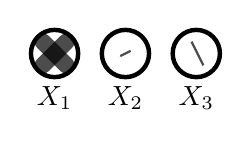
\begin{tikzpicture}[scale = .3]
      \draw[ultra thick] (0,0) circle (1cm);
      \draw[ultra thick] (3,0) circle (1cm);
      \draw[ultra thick] (6,0) circle (1cm);
      \node[below] at (0,-1) {$X_1$};
      \node[below] at (3,-1) {$X_2$};
      \node[below] at (6,-1) {$X_3$};
      % Marking the circles carelessly
      \draw[black,line width=6pt,line cap=round,opacity=.7] (0.5,-0.5) -- (-0.5,0.5);
      % \draw[black!70!white,thick] (3.1,-0.3) -- (2.7,0.5);
      \draw[black!70!white,thick] (5.8,0.5) -- (6.3,-0.5);
      % \draw[black,thick,line width=6pt,line cap=round,opacity=.7] (5.5,-0.5) -- (6.5,0.5);
      \draw[black,thick,line width=6pt,line cap=round,opacity=.7] (0.5,0.5) -- (-0.5,-0.5);
      \draw[black,thick,line cap=round,opacity=.7] (3.2,0.1) -- (2.8,-0.1);
      % \draw[black,thick,line width=6pt,line cap=round,opacity=.7] (5.5,0.5) -- (5.5,-0.5);
    \end{tikzpicture}
  \end{center}
  Shading may be incomplete, and there may be errent marks.
  We can use a \link[neural network]{https://en.wikipedia.org/wiki/Neural_network} to help solve this problem.
  This might sound really complicated, but at the end of the day, a neural network is just a matrix.


  Since the marks are incomplete, we visualize the input as continuous
  random variables $X_1$, $X_2$, and $X_3$; where a value of $1$ for
  $X_i$ would represent ``completely shaded'' and a value of $0$ for
  $X_i$ would represent completely unshaded. We can express these random
  variables as a column vector $\vec{X}$. Moreover, we may write the
  ``answer'' of whether the pattern is shaded correctly, using a column
  vector $\vec{Y}$, with two entries, also random variables $Y_1$ and
  $Y_2$, where $Y_1$ is the probability that the circles are filled in
  correctly, and $Y_2$ is the probability they are not.
  \[
    \vec{X} = \begin{pmatrix} X_1 \\ X_2 \\ X_3 \end{pmatrix} \qquad \vec{Y} = \begin{pmatrix} Y_1 \\ Y_2 \end{pmatrix}
  \]
  A matrix $H$ represents the neural network, say
  \[
    H = \begin{pmatrix}
      0.375 & -0.125 & -0.125 \\
      0.125 & 0.625 & 0.625
    \end{pmatrix},
  \]
  and we find $\vec{Y}$ by
  \[
    \vec{Y} =
    H\vec{X} =
    \begin{pmatrix}
      0.288 \\
      0.163
    \end{pmatrix},
  \]
  for some $X$. Interpret this result and represent this matrix
  equation as a system of equations.
  \begin{explanation}
    Since vector
    \[
      \vec{Y} =
      \begin{pmatrix}
        \answer[given]{0.288} \\
        \answer[given]{0.163}
      \end{pmatrix},
    \]
    we see that the drawn pattern, represented by $X_1$, $X_2$, and
    $X_3$, is likely the
    \wordChoice{\choice[correct]{correct}\choice{incorrect}} pattern.
    Writing
    \[
      H\vec{X} =
      \begin{pmatrix}
        0.288 \\
        0.163
      \end{pmatrix}
    \]
    corresponds to the system of equations:
    \begin{align*}
      \left(\answer[given]{0.375}\right)X_1 + \left(\answer[given]{-0.125}\right) X_2 + \left(\answer[given]{-0.125}\right) X_3 &= 0.288 \\
      \left(\answer[given]{0.125}\right)X_1 + \left(\answer[given]{0.625}\right) X_2 + \left(\answer[given]{0.625}\right)X_3 &= 0.163
    \end{align*}
  \end{explanation}
\end{example}



Networks, not to be confused with \textit{neural} networks, have
numerous applications, from traffic networks to circuits, to actual computer networks.



\begin{example}[Network Analysis]
  A network is composed of nodes and directed edges, describing a
  ``flow'' into each node and a ``flow'' out of each node.
  \begin{center}
    \begin{tikzpicture}[scale=2]
      \begin{scope}[very thick,decoration={
          markings,
          mark=at position 0.5 with {\arrow{>}}}
        ]
        \tikzset{vertex/.style = {shape=circle,draw,minimum size=1.5em}}
        % vertices
        \node[vertex] (a) at  (-1,1.7) {$A$};
        \node[vertex] (b) at  (1,1.7) {$B$};
        \node[vertex] (c) at  (0,0) {$C$};
        % edges
        \draw[postaction={decorate}] (a) to[bend right] node[below left] {$30$}  (c);
        \draw[postaction={decorate}] (c) to[bend right] node[below right] {$40$} (b);
        \draw[postaction={decorate}] (b) to[bend right] node[above] {$20$} (a);


        \draw[postaction={decorate}] (a) to[bend left] node[below left] {$2x_2$} (c);
        \draw[postaction={decorate}] (a) to[bend right] node[above] {$x_1$} (b);
        \draw[postaction={decorate}] (b) to[bend right] node[below right] {$x_3$} (c);
      \end{scope}
    \end{tikzpicture}
  \end{center}
  It is of critical importance that \textbf{flow into a node equals the
    flow out of a node}. So for example, the flow into node $A$ above is
  $20$. However, the flow out of $A$ is $x_{1} + 2x_{2} + 30$. Hence
  \[
    20  = x_{1} + 2x_{2} + 30.
  \]
  Write an equation for the remaining nodes and express the system of
  equations as a matrix multipled by a vector.
  \begin{explanation}
    First we write the equations, remember that the flow into a node
    equals the flow out of a node:
    \begin{align*}
      20 &= x_{1} + 2x_{2} + 30 & & (A)\\
      x_{1} + \left(\answer[given]{40}\right) &= x_{3} + 20 & & (B) \\
      2x_{2} + x_{3} + \left(\answer[given]{30}\right) &= 40  & & (C)
    \end{align*}
    leading to:
    \begin{align*}
      x_{1}+2x_{2} &= \answer[given]{-10}\\
      x_{1} -x_{3}&= \answer[given]{-20}\\
      2x_{2} + x_{3}  &= \answer[given]{10}
    \end{align*}
    %% TK: The following may be tedious to code but column alignment
    %% makes it instantly clear to write out the coefficient matrix
    %% without errors. Any suggestions on pretty typesetting of a system
    %% of equations are welcome.
    % \begin{equation*}
    %   \begin{array}{*{7}{@{}c@{}}}
    %     x_1  & {}+{}  & 2 x_2  &    &      & {}\mathrel{=}{}  & \answer[given]{-10} \\
    %     x_1  &    &        & {}-{}  & x_3  & {}\mathrel{=}{}  & \answer[given]{-20} \\
    %     &    & 2 x_2  & {}+{}  & x_3  & {}\mathrel{=}{}  & \answer[given]{10}
    %   \end{array}
    % \end{equation*}
    Setting
    \[
      A = \begin{pmatrix}
        1 & 2 & 0\\
        1 & \answer[given]{0} & -1 \\
        \answer[given]{0} & \answer[given]{2} & 1
      \end{pmatrix},
      \quad
      \vec{x} =
      \begin{pmatrix}
        x_1\\
        x_2\\
        x_3
      \end{pmatrix},
      \quad
      \vec{b} =
      \begin{pmatrix}
        \answer[given]{-10}\\
        \answer[given]{-20}\\
        \answer[given]{10}
      \end{pmatrix},
    \]
    we may express this system of equations as $A\vec{x} = \vec{b}$.
  \end{explanation}
\end{example}













\section{Multiplying matrices}



Matrix multiplication may seem strange at first. In fact, only certain
matrices can be multiplied together. As a general rule, we can only
multiply a $m \times n$ matrix by a $k \times \l$ matrix if $n=k$. That is, the
number of columns in the first matrix must equal the number of rows in
the second matrix:
%% TK: The original explanation is not clear. Though verbose, why
%% don't we write out clearly what is meant? We are backing it up with
%% a nice diagram below anyway.
% That is, if \textbf{the middle two numbers match}: <-- not clear.
\[
  \begin{matrix}
    \begin{pmatrix}
      \bullet & \bullet & \bullet & \bullet & \bullet \\
      \bullet & \bullet & \bullet & \bullet & \bullet \\
    \end{pmatrix}
    &
      \begin{pmatrix}
        \bullet & \bullet & \bullet \\
        \bullet & \bullet & \bullet \\
        \bullet & \bullet & \bullet \\
        \bullet & \bullet & \bullet \\
        \bullet & \bullet & \bullet
      \end{pmatrix}
    &=&
        \begin{pmatrix}
          \bullet & \bullet & \bullet \\
          \bullet & \bullet & \bullet
        \end{pmatrix} \\
    &&&\\
    \begin{pmatrix}
      \boldsymbol{{\color{penColor2} m} \times {\color{penColor6} \cancel n}} \\
      \text{matrix}
    \end{pmatrix}
    &
      \begin{pmatrix}
        \boldsymbol{{\color{penColor6} \cancel n} \times {\color{penColor4} \l}} \\
        \text{matrix}
      \end{pmatrix}
    &=&
        \begin{pmatrix}
          \boldsymbol{{\color{penColor2} m} \times {\color{penColor4}\l}} \\
          \text{matrix}
        \end{pmatrix}
  \end{matrix}
\]
% The product then turns out to be a matrix of size $m\times \ell$, \textbf{the
% outside numbers}.
Note that the number of the rows of the product equals that of the
first matrix, and the number of columns of the product equals that of
the second matrix.

\begin{question}
  Given three matrices
  \[
    A =\begin{pmatrix}
      1 & -2 & 3 \\
      0 & 5 & -6 \\
      -7 & 8 & 0
    \end{pmatrix},\quad B =\begin{pmatrix}
      1 & 0 \\
      -3 & 4 \\
      5 & -6
    \end{pmatrix}, \quad C =\begin{pmatrix}
      0 & -2 & 3 \\
      4 & 0 & -6
    \end{pmatrix},
  \]
  which of the following make sense?
  \begin{selectAll}\pdfOnly{\begin{multicols}{3}}
      \choice[correct]{$AA$}
      \choice[correct]{$AB$}
      \choice{$AC$}
      \choice{$BA$}
      \choice{$BB$}
      \choice[correct]{$BC$}
      \choice[correct]{$CA$}
      \choice[correct]{$CB$}
      \choice{$CC$}
      \pdfOnly{\end{multicols}}
  \end{selectAll}
  \begin{question}
    What are the dimensions of the products?
    \pdfOnly{\begin{multicols}{3}}
      \begin{enumerate}
      \item $AA$\begin{prompt}~is a $\answer{3}\times\answer{3}$ matrix.\end{prompt}
      \item $AB$\begin{prompt}~is a $\answer{3}\times\answer{2}$ matrix.\end{prompt}
      \item $BC$\begin{prompt}~is a $\answer{3}\times\answer{3}$ matrix.\end{prompt}
      \item $CA$\begin{prompt}~is a $\answer{2}\times\answer{3}$ matrix.\end{prompt}
      \item $CB$\begin{prompt}~is a $\answer{2}\times\answer{2}$ matrix.\end{prompt}
      \item $ABC$\begin{prompt}~is a $\answer{2}\times\answer{2}$ matrix.\end{prompt}
      \end{enumerate}
      \pdfOnly{\end{multicols}}
  \end{question}
\end{question}


%% We'll give several different explanations and interpretations of this
%% computation.

%% \subsection{As an extension of the dot product}
We can extend the concept of the dot product to explain how to
multiply a matrix by another matrix. Here is an example:
\begin{align*}AB &= \begin{pmatrix}
  a_{1,1} & a_{1,2}\\
  a_{2,1} & a_{2,2}
\end{pmatrix}
                   \begin{pmatrix}
                     b_{1,1} & b_{1,2}\\
                     b_{2,1} & b_{2,2}
                   \end{pmatrix}\\
                 &= \begin{pmatrix}
                   \row_1(A)^\transpose \dotp\col_1(B) & \row_1(A)^\transpose\dotp\col_2(B)\\
                   \row_2(A)^\transpose \dotp\col_1(B) & \row_2(A)^\transpose\dotp\col_2(B)
                 \end{pmatrix}\\
                 &= \begin{pmatrix}
                   a_{1,1}b_{1,1} + a_{1,2}b_{2,1} & a_{1,1}b_{1,2}+ a_{1,2}b_{2,2}\\
                   a_{2,1}b_{1,1} + a_{2,2}b_{2,1} & a_{2,1}b_{1,2} + a_{2,2}b_{2,2}
                 \end{pmatrix}
\end{align*}
We attempt to describe the structure of this product in the diagram below:
\begin{center}
  \begin{tikzpicture}[]
    \matrix (matA) [%
    matrix of nodes,
    left delimiter={(},right delimiter={)}
    ]
    {%
      \phantom{$\bullet$} & \phantom{$\bullet$} & \phantom{$\bullet$} & \phantom{$\bullet$} & \phantom{$\bullet$}\\
      \phantom{$\bullet$} & \phantom{$\bullet$} & \phantom{$\bullet$} & \phantom{$\bullet$} & \phantom{$\bullet$}\\
    };
    \draw[black,ultra thick,line cap=round] (matA-1-1.west)  -- (matA-1-5.east);
    \draw[black,ultra thick,line cap=round] (matA-2-1.west) -- (matA-2-5.east);

    \matrix (matB) [%
    matrix of nodes,right= of matA,
    left delimiter={(},right delimiter={)}
    ]
    {%
      \phantom{$\bullet$} & \phantom{$\bullet$} &\phantom{$\bullet$} \\\phantom{$\bullet$} & \phantom{$\bullet$} & \phantom{$\bullet$} \\  \phantom{$\bullet$} & \phantom{$\bullet$} & \phantom{$\bullet$} \\\phantom{$\bullet$} & \phantom{$\bullet$} & \phantom{$\bullet$} \\ \phantom{$\bullet$} & \phantom{$\bullet$} & \phantom{$\bullet$} \\
    };
    \draw[black,ultra thick,line cap=round] (matB-1-1.north)  -- (matB-5-1.south);
    \draw[black,ultra thick,line cap=round] (matB-1-2.north) -- (matB-5-2.south);
    \draw[black,ultra thick,line cap=round] (matB-1-3.north) -- (matB-5-3.south);

    \node[right=2ex of matB] {$=\begin{pmatrix}
      \boldsymbol{-}^\transpose\dotp\boldsymbol{|} & \boldsymbol{-}^\transpose\dotp\boldsymbol{|} &\boldsymbol{-}^\transpose\dotp\boldsymbol{|} \\\boldsymbol{-}^\transpose\dotp\boldsymbol{|} & \boldsymbol{-}^\transpose\dotp\boldsymbol{|} &  \boldsymbol{-}^\transpose\dotp\boldsymbol{|}
    \end{pmatrix}$};
\end{tikzpicture}
\end{center}
Above the strange symbols
``$\boldsymbol{-}^\transpose\dotp\boldsymbol{|}$'' are supposed to
represent the transpose of the rows of $A$ being dotted with the
columns of $B$. Quite generally, if $A$ is an $m\times n$ matrix and
$B$ is a $n\times \l$ matrix, then $C = AB$ is a $m\times \l$ matrix and
\[
  c_{ij} = \row_i(A)^\transpose\dotp \col_j(B).
\]
\begin{question} If
  \[
    A = \begin{pmatrix}
      1 & -2 & 3 & 0 & -1 \\
      4 & 0 & -5 & 6 & -7
    \end{pmatrix}\quad\text{and}\quad
    B=
    \begin{pmatrix}
      1 & -2 & 3 \\
      0 & 5 & -6 \\
      -7 & 8 & 0 \\
      4 & -5 & 6 \\
      -1 & 2 & 1
    \end{pmatrix}
  \]
  and $C = AB$, what is $c_{2,3}$?
  \begin{prompt}
    \[
      c_{2,3} = \answer{41}
    \]
  \end{prompt}
\end{question}












%% \subsection{Columns of the product}



%% Another viewpoint is to build the product as columns.
%% \begin{align*}AB &= \begin{pmatrix}
  %%   a_{1,1} & a_{1,2}\\
%% a_{2,1} & a_{2,2}
%% \end{pmatrix}
%% \begin{pmatrix}
%% b_{1,1} & b_{1,2}\\
%% b_{2,1} & b_{2,2}
%% \end{pmatrix}\\
%% &= \begin{pmatrix}
%% \col_1(A)b_{1,1} + \col_2(A) b_{2,1} & \col_1(A)b_{1,2} + \col_2(A) b_{2,2}
%% \end{pmatrix}\\
%% &= \begin{pmatrix}
%% \begin{pmatrix}a_{1,1} \\ a_{2,1}\end{pmatrix}b_{1,1} + \begin{pmatrix}a_{1,2} \\ a_{2,2}\end{pmatrix}b_{2,1} & \begin{pmatrix}a_{1,1} \\ a_{2,1}\end{pmatrix}b_{1,2} + \begin{pmatrix}a_{1,2} \\ a_{2,2}\end{pmatrix}b_{2,2}
%% \end{pmatrix}\\
%% &= \begin{pmatrix}
%% a_{1,1}b_{1,1} + a_{1,2}b_{2,1} & a_{1,1}b_{1,2}+ a_{1,2}b_{2,2}\\
%% a_{2,1}b_{1,1} + a_{2,2}b_{2,1} & a_{2,1}b_{1,2} + a_{2,2}b_{2,2}
%% \end{pmatrix}
%% \end{align*}

%% We attempt to describe the structure of this product in the diagram below:
%% \begin{center}
%% \begin{tikzpicture}[]
%%      \matrix (matA) [%
%%        matrix of nodes,
%%        left delimiter={(},right delimiter={)}
%%      ]
%%       {%
%%         \phantom{$\bullet$} & \phantom{$\bullet$} & \phantom{$\bullet$} & \phantom{$\bullet$} & \phantom{$\bullet$}\\
%%         \phantom{$\bullet$} & \phantom{$\bullet$} & \phantom{$\bullet$} & \phantom{$\bullet$} & \phantom{$\bullet$}\\
%%       };
%%       \draw[black,ultra thick,line cap=round] (matA-1-1.north)  -- (matA-2-1.south);
%%       \draw[black,ultra thick,line cap=round] (matA-1-2.north)  -- (matA-2-2.south);
%%       \draw[black,ultra thick,line cap=round] (matA-1-3.north)  -- (matA-2-3.south);
%%       \draw[black,ultra thick,line cap=round] (matA-1-4.north)  -- (matA-2-4.south);
%%       \draw[black,ultra thick,line cap=round] (matA-1-5.north)  -- (matA-2-5.south);

%%       \matrix (matB) [%
%%         matrix of nodes,right=of matA,
%%        left delimiter={(},right delimiter={)}
%%      ]
%%       {%
%%         $\bullet$ & $\bullet$ &$\bullet$ \\$\bullet$ & $\bullet$ & $\bullet$ \\  $\bullet$ & $\bullet$ & $\bullet$ \\$\bullet$ & $\bullet$ & $\bullet$ \\ $\bullet$ & $\bullet$ & $\bullet$ \\
%%       };
%%       \draw[black!20!white,line width=1ex,line cap=round] (matB-1-1.north)  -- (matB-5-1.south);
%%       \draw[black!20!white,ultra thick,line width=1ex,line cap=round] (matB-1-2.north) -- (matB-5-2.south);
%%       \draw[black!20!white,ultra thick,line width=1ex,line cap=round] (matB-1-3.north) -- (matB-5-3.south);

%%       \node[right=2ex of matB] {$=\begin{pmatrix}
%%   \boldsymbol{\Big|\mkern-4mu\cdot\mkern-4mu\Big|\mkern-4mu\cdot\mkern-4mu\Big|\mkern-4mu\cdot\mkern-4mu\Big|\mkern-4mu\cdot\mkern-4mu\Big|\cdot} & \boldsymbol{\Big|\mkern-4mu\cdot\mkern-4mu\Big|\mkern-4mu\cdot\mkern-4mu\Big|\mkern-4mu\cdot\mkern-4mu\Big|\mkern-4mu\cdot\mkern-4mu\Big|\cdot} & \boldsymbol{\Big|\mkern-4mu\cdot\mkern-4mu\Big|\mkern-4mu\cdot\mkern-4mu\Big|\mkern-4mu\cdot\mkern-4mu\Big|\mkern-4mu\cdot\mkern-4mu\Big|\cdot} \\
%%         \end{pmatrix}$};
%%       \matrix (matBp) [%
%%         matrix of nodes,right=of matA,
%%        left delimiter={(},right delimiter={)}
%%      ]
%%       {%
%%         $\bullet$ & $\bullet$ &$\bullet$ \\$\bullet$ & $\bullet$ & $\bullet$ \\  $\bullet$ & $\bullet$ & $\bullet$ \\$\bullet$ & $\bullet$ & $\bullet$ \\ $\bullet$ & $\bullet$ & $\bullet$ \\
%%       };
%% \end{tikzpicture}
%% \end{center}
%% Above the strange symbols
%% ``$\boldsymbol{\Big|\mkern-4mu\cdot\mkern-4mu\Big|\mkern-4mu\cdot\mkern-4mu\Big|\mkern-4mu\cdot\mkern-4mu\Big|\mkern-4mu\cdot\mkern-4mu\Big|\cdot}$''
%% are supposed to represent the sum of the columns of $A$ each multipled
%% by an element of a column of $B$.  Quite generally, if $A$ is an
%% $m\times n$ matrix and $B$ is a $n\times \l$ matrix, and $C = AB$ is a
%% $m\times \l$ matrix, then
%% \[
%% \col_i(C) = \sum_{k=1}^n \col_k(A)b_{k,i}
%% \]
%% that is,
%% \begin{align*}
%%   C &= \begin{pmatrix} \col_1(C) & \col_2 (C) & \cdots & \col_{\l}(C) \end{pmatrix}\\
%%   &=  \begin{pmatrix} \sum_{k=1}^n \col_k(A)b_{k,1} & \sum_{k=1}^n \col_k(A)b_{k,2} & \cdots & \sum_{k=1}^n \col_k(A)b_{k,\l}\end{pmatrix}
%% \end{align*}
%% \begin{question} If
%%   \[
%%   A = \begin{pmatrix}
%% 1 & -2 & 3 & 0 & -1 \\
%% 4 & 0 & -5 & 6 & -7
%%   \end{pmatrix}\quad\text{and}\quad
%%   B=
%%   \begin{pmatrix}
%% 1 & -2 & 3 \\
%% 0 & 5 & -6 \\
%% -7 & 8 & 0 \\
%% 4 & -5 & 6 \\
%% -1 & 2 & 1
%% \end{pmatrix}
%%   \]
%%   and $C = AB$, what is $\col_2(C)$?
%%   %\begin{prompt}
%%     \[
%%     \col_2(C) =  \col_1(A)b_{1,2} +  \col_2(A)b_{2,2}+  \col_3(A)b_{3,2} + \col_4(A) b_{4,2} + \col_5(A) b_{5,2}
%%     \]
%%   %\end{prompt}
%% \end{question}











%% \subsection{Rows of the product}


%% \begin{align*}AB &= \begin{pmatrix}
%% a_{1,1} & a_{1,2}\\
%% a_{2,1} & a_{2,2}
%% \end{pmatrix}
%% \begin{pmatrix}
%% b_{1,1} & b_{1,2}\\
%% b_{2,1} & b_{2,2}
%% \end{pmatrix}\\
%% &= \begin{pmatrix}
%% a_{1,1}\row_1(B) + a_{1,2}\row_2(B) \\ a_{2,1}\row_1(B) +  a_{2,2}\row_2(B)
%% \end{pmatrix}\\
%% &= \begin{pmatrix}
%% a_{1,1}\begin{pmatrix} b_{1,1} & b_{1,2}\end{pmatrix} + a_{1,2}\begin{pmatrix} b_{2,1} & b_{2,2}\end{pmatrix} \\ a_{2,1}\begin{pmatrix} b_{1,1} & b_{1,2}\end{pmatrix} +  a_{2,2}\begin{pmatrix} b_{2,1} & b_{2,2}\end{pmatrix}
%% \end{pmatrix}\\
%% &= \begin{pmatrix}
%% a_{1,1}b_{1,1} + a_{1,2}b_{2,1} & a_{1,1}b_{1,2}+ a_{1,2}b_{2,2}\\
%% a_{2,1}b_{1,1} + a_{2,2}b_{2,1} & a_{2,1}b_{1,2} + a_{2,2}b_{2,2}
%% \end{pmatrix}
%% \end{align*}

%% Quite generally, if $A$ is an $m\times n$ matrix and $B$ is a $n\times
%% \l$ matrix, and $C = AB$ is a $m\times \l$ matrix, then
%% \[
%% \row_i(C) = \sum_{k=1}^n a_{i,k}\row_k(B)
%% \]
%% that is,
%% \[
%%   C = \begin{pmatrix} \row_1(C) \\ \row_2 (C) \\ \vdots \\ \row_{m}(C) \end{pmatrix}
%%   =  \begin{pmatrix} \sum_{k=1}^n a_{1,k}\row_k(B) \\ \sum_{k=1}^n a_{2,k}\row_k(B) \\ \vdots \\ \sum_{k=1}^n a_{m,k}\row_k(B)\end{pmatrix}
%% \]















\begin{question}
For the following matrices, find $AB$ and $BA$.
\[
A= \begin{pmatrix}
5 & 0 \\
2 & 1
\end{pmatrix}, \quad B =
\begin{pmatrix}
3 & -1 \\
2 & 0
\end{pmatrix}
\]
\begin{prompt}
\[
AB =\begin{pmatrix}
\answer[given]{15} & \answer[given]{-5}\\
\answer[given]{8} & \answer[given]{-2}
\end{pmatrix}
\]

\[
BA = \begin{pmatrix}
\answer[given]{13} & \answer[given]{-1}\\
\answer[given]{10} & \answer[given]{0}
\end{pmatrix}
\]
\end{prompt}
Do the two multiplications give the same result?
\begin{prompt}
  \begin{multipleChoice}
    \choice{Yes.}
    \choice[correct]{No.}
  \end{multipleChoice}
\end{prompt}
\end{question}


\begin{example}[Matrix Multiplication]
  Let:
  \[
  A = \begin{pmatrix}
    1 & -1 & 0\\
    2 & 0 & 4 \\
    5 & 3 & 1
  \end{pmatrix}
  \quad\text{and}\quad B =
  \begin{pmatrix}
    5 & 1 & 0\\
    -1 & -2 & 0\\
    1 & 0 & 2
  \end{pmatrix}
  \]
  Compute $AB$.
  \begin{explanation}
    Write with me, note it is important to write the matrices neatly
    and put enough space between entries. We start by writing the sum:
    \begin{align*}
      AB &= \begin{pmatrix}
        (1)\left(\answer[given]{5}\right) + (-1)\left(\answer[given]{-1}\right)+ (0)\left(\answer[given]{1}\right) & (-1)\left(\answer[given]{-1}\right) + (-1)\left(\answer[given]{2}\right)+ 0 & 0 + 0+ 0\\
        10 + 0 + 4 & 2 + 0+0 & 0 + 0+8\\
        25+ (-3) + 1 & 5 + -6+0 & 0 + 0+ 2
      \end{pmatrix}\\
      &= \begin{pmatrix}
        \answer[given]{6} &  \answer[given]{3} &  \answer[given]{0}\\
         \answer[given]{14}&  \answer[given]{2} &  \answer[given]{8}\\
         \answer[given]{23} &  \answer[given]{-1} &  \answer[given]{2}
      \end{pmatrix}
    \end{align*}
    Matrix multiplication is not difficult, you just need to be
    careful.
  \end{explanation}
\end{example}




%% Since vectors can be viewed as matrices, matrix multiplication applies
%% to vectors too.  If $\vec{x}$ and $\vec y$ are $n$-vectors with
%% \begin{itemize}
%% \item $\vec{x}$ expressed as a row,
%% \item $\vec{y}$ expressed as a column,
%% \end{itemize}
%% then $\vec{y}\vec{x}$ can be inteperted as either a $n\times 1$
%% matrix multiplied by a row vector or a column vector multipled by a
%% $1\times n$ matrix. In either case the answers are the same, and will be a
%% $n\times n$ matrix. This particular form of a vector product in which a
%% column vector is multiplied by a row vector resulting in a matrix is
%% called the \dfn{outer product}.

%% TK: How above we assume that x and y are both column n-vectors and
%% describe two vector products, namely, the inner product x' * y and
%% the outer product x * y'? (v' denotes v-transpose)
Since vectors can be viewed as matrices, matrix multiplication applies
to vectors too. Suppose $\vec{x}$ and $\vec y$ are column $n$-vectors.
\begin{description}
\item[Inner product.] The product $\vec{x}\dotp\vec{y} =
  \vec{x}^\transpose \vec{y}$ can be interpreted as either a $1 \times
  n$ matrix multiplied by an appropriately sized column vector or a
  row vector multiplied by an $n \times 1$ matrix. Either case results
  in a $1 \times 1$ matrix, that is, a scalar. This form of a vector
  product in which a row vector is multiplied by a column vector
  producing a scalar is called the \dfn{inner product}. This is
  another name for the familiar dot product.
\item[Outer product.] The product $\vec{x} \vec{y}^\transpose$ can be
  inteperted as either a $n\times 1$ matrix multiplied by a row vector or a
  column vector multipled by a $1\times n$ matrix. In either case the
  answers are the same, and will be a $n\times n$ matrix. This particular
  form of a vector product in which a column vector is multiplied by a
  row vector resulting in a matrix is called the \dfn{outer product}.
\end{description}



We'll use the outer product in our next example.

\begin{example}[Distributions]
  We encode a vectors with various distributions. For example the
  entries of vector $\vec{n}$ follow a normal distribution
  \[
  \vec{n}^\transpose =\begin{pmatrix} 0.11 & 0.22 & 0.39 & 0.58 & 0.74 & 0.8 & 0.74 & 0.58 & 0.39 & 0.22 & 0.11 \end{pmatrix}
  \]
  We can plot the entries, and describe them as a grayscale image
  \begin{center}
    \newcommand{\matrixData}{{
        {0.11, 0.22, 0.39, 0.58, 0.74, 0.8, 0.74, 0.58, 0.39, 0.22, 0.11}
    }}
    \begin{tikzpicture}[xscale=.5]
      \begin{scope}[yscale=2.5]
        % Draw the axes
        \draw[->] (0,0) -- (12,0);
        \draw[->] (0,0) -- (0,1);
        \node at (2,.6) {$\vec{n}$};
        % Plot the data points and lines between them
        \draw[thick] (1,0.11) -- (2,0.22) -- (3,0.39) -- (4,0.58) -- (5,0.74)
        -- (6,0.80) -- (7,0.74) -- (8,0.58) -- (9,0.39)
        -- (10,0.22) -- (11,0.11);
      \end{scope}
      \begin{scope}[yscale=.5]
      \foreach \x in {0, 1, ..., 10} {
          \pgfmathsetmacro\val{\matrixData[0][\x]}
          \fill[black, opacity={1-\val}] (.5+\x, -.5) rectangle (\x+1.5, -1.5);
          \draw (.5+\x, -.5) rectangle (\x+1.5, -1.5);
      }
      \end{scope}
    \end{tikzpicture}
  \end{center}
  We can also encode a skewed normal distribution
  \[
  \vec{s}^\transpose =\begin{pmatrix} 0 & 0.01 & 0.07 & 0.26 & 0.61 & 1 & 1.15 & 0.95 & 0.57 & 0.26 & 0.09\end{pmatrix}
  \]
 Plotting the entries, and describing them with grayscale we find:
  \begin{center}
    \newcommand{\matrixData}{{
        {0., 0.01, 0.07, 0.26, 0.61, 1., 1.15, 0.95, 0.57, 0.26, 0.09}
    }}
    \begin{tikzpicture}[xscale=.5]
      \begin{scope}[yscale=2.5]
        % Draw the axes
        \draw[->] (0,0) -- (12,0);
        \draw[->] (0,0) -- (0,1);
        \node at (2,.6) {$\vec{s}$};
        % Plot the data points and lines between them
        \draw[thick] (1,0) -- (2,0.01) -- (3,0.07) -- (4,0.26) -- (5,0.61)
                 -- (6,1) -- (7,1.15) -- (8,0.95) -- (9,0.57) -- (10,0.26)
                 -- (11,0.09);
      \end{scope}
      \begin{scope}[yscale=.5]
      \foreach \x in {0, 1, ..., 10} {
          \pgfmathsetmacro\val{\matrixData[0][\x]}
          \fill[black, opacity={1-\val}] (.5+\x, -.5) rectangle (\x+1.5, -1.5);
          \draw (.5+\x, -.5) rectangle (\x+1.5, -1.5);
      }
      \end{scope}
    \end{tikzpicture}
  \end{center}
  Let $P = \vec{n}\vec{s}^\transpose$. Compute $p_{6,7}$ and interpret
  the matrix $P$ itself.
  \begin{explanation}
    Viewing $\vec{n}$ as a $11\times 1$ matrix and
    $\vec{s}^\transpose$ as a $1 \times 11$ matrix, the (outer) product
    $\vec{n}\vec{s}^\transpose$ will be an
    $\answer[given]{11}\times\answer[given]{11}$ matrix, and have
    $\answer[given]{121}$ entries. $p_{6,7}$ is
    $\answer[given]{0.92}$.

    The product $P$ is now a distribution of two variables, and can be
    viewed as the following grayscale image':
    \begin{center}
      \newcommand{\matrixData}{{
          {0,0,0.01,0.03,0.07,0.11,0.13,0.1,0.06,0.03,0.01},
          {0,0,0.02,0.06,0.13,0.22,0.25,0.21,0.13,0.06,0.02},
          {0,0,0.03,0.1,0.24,0.39,0.45,0.37,0.22,0.1,0.04},
          {0,0.01,0.04,0.15,0.35,0.58,0.67,0.55,0.33,0.15,0.05},
          {0,0.01,0.05,0.19,0.45,0.74,0.85,0.7,0.42,0.19,0.07},
          {0,0.01,0.06,0.21,0.49,0.8,0.92,0.76,0.46,0.21,0.07},
          {0,0.01,0.05,0.19,0.45,0.74,0.85,0.7,0.42,0.19,0.07},
          {0,0.01,0.04,0.15,0.35,0.58,0.67,0.55,0.33,0.15,0.05},
          {0,0,0.03,0.1,0.24,0.39,0.45,0.37,0.22,0.1,0.04},
          {0,0,0.02,0.06,0.13,0.22,0.25,0.21,0.13,0.06,0.02},
          {0,0,0.01,0.03,0.07,0.11,0.13,0.1,0.06,0.03,0.01}
      }}
      \newcommand{\skewData}{{
           {0., 0.01, 0.07, 0.26, 0.61, 1., 1.15, 0.95, 0.57, 0.26, 0.09}
      }}
      \newcommand{\normData}{{
          {0.11, 0.22, 0.39, 0.58, 0.74, 0.8, 0.74, 0.58, 0.39, 0.22, 0.11}
      }}
      \begin{tikzpicture}[scale=.5]
      \foreach \y in {0, ...,10} {
        \foreach \x in {0, 1, ..., 10} {
          \pgfmathsetmacro\val{\matrixData[\y][\x]}
          \fill[black, opacity={1-\val}] (\x, -\y) rectangle (\x+1, -\y-1);
          \draw (\x, -\y) rectangle (\x+1, -\y-1);
        }
      }

      \foreach \x in {0, 1, ..., 10} {
          \pgfmathsetmacro\val{\skewData[0][\x]}
          \fill[black, opacity={1-\val}] (\x, -11.5) rectangle (\x+1, -12.5);
          \draw (\x, -11.5) rectangle (\x+1, -12.5);
      }

      \foreach \x in {0, 1, ..., 10} {
        \pgfmathsetmacro\val{\normData[0][\x]}
        \fill[black, opacity={1-\val}] (-.5,-\x) rectangle (-1.5,-\x-1);
        \draw (-.5,-\x) rectangle (-1.5,-\x-1);
      }
      \node at (-2,-5.5) {$\vec{n}^\transpose$};
      \node at (5.5,-13) {$\vec{s}$};

    \end{tikzpicture}
  \end{center}
    From the picture above, we can visually confirm that our
    computation from before is correct.
    \end{explanation}
\end{example}









\section{Matrices transform data}

So far we have discussed ways matrices encode data. However, they also
transform data.


\begin{example}[RGB to Luminance and Chrominance]
  A color RGB image is encoded as three matrices,
  \begin{center}
    \begin{tikzpicture}
    \node at (-2.5,2)  {
\includegraphics[width=3cm]{catface.jpg}};
    \node at (2.5,2)   {
\includegraphics[width=3cm]{catfaceB.jpg}};
    \node at (-2.5,-2) {
\includegraphics[width=3cm]{catfaceR.jpg}};
    \node at (2.5,-2)  {
\includegraphics[width=3cm]{catfaceG.jpg}};
    \draw[line width =3mm, blue,->] (.8,2)--(-.8,2);
    \draw[line width =3mm, red,->] (-2.5,-.8)--(-2.5,.8);
    \draw[line width =3mm, green,->] (.8,-.8)--(-.8,.8);
    \node at (-2.5,-3.5) {red channel};
    \node at (2.5,-3.5) {green channel};
    \node at (2.5,.5) {blue channel};
    \end{tikzpicture}
  \end{center}
  One representing red, green, and blue. Each pixel of the full color
  image is a $3$-vector. Note, for this picture, each of the
  components is essentially equally intricate and detailed. However,
  another popular encoding method is \link[Luminance and Chrominance
    ($YC_BC_R$)]{https://en.wikipedia.org/wiki/YCbCr}.  One method to
  transform RGB color to $YC_BC_R$ is to write
  \[
  \begin{pmatrix}
    0\\
    128\\
    128
  \end{pmatrix}
  +
  \begin{pmatrix}
        0.299  &  0.587  &  0.114 \\
   -0.169 & -0.331 &  0.5 \\
    0.5   & -0.419 & -0.081
  \end{pmatrix}
  \begin{pmatrix}
    R\\ G \\ B
  \end{pmatrix}
  =
  \begin{pmatrix}
  Y\\
  C_B\\
  C_R
  \end{pmatrix}.
  \]
  Observe, when we do this transformation to the image of our cat
  above:
    \begin{center}
    \begin{tikzpicture}
    \node at (-2.5,2)  {
\includegraphics[width=3cm]{catface.jpg}};
    \node at (2.5,2)   {
\includegraphics[width=3cm]{catfaceCr.jpg}};
    \node at (-2.5,-2) {
\includegraphics[width=3cm]{catfaceY.jpg}};
    \node at (2.5,-2)  {
\includegraphics[width=3cm]{catfaceCb.jpg}};
    \draw[line width =3mm, gray,->] (.8,2)--(-.8,2);
    \draw[line width =3mm, black,->] (-2.5,-.8)--(-2.5,.8);
    \draw[line width =3mm, gray,->] (.8,-.8)--(-.8,.8);
    \node at (-2.5,-3.5) {$Y$ channel};
    \node at (2.5,-3.5) {$C_B$ channel};
    \node at (2.5,.5) {$C_R$ channel};
    \end{tikzpicture}
    \end{center}
    Note how little detail is showing in the $C_b$ and $C_r$ channels.


    In the RGB color image, the pixel at $(229,405)$ has an RGB value of
    \[
    \begin{pmatrix} 40 & 72 & 60 \end{pmatrix}^\transpose
    \]
    What are the $YC_BC_R$ values for this pixel?
    \begin{explanation}
      To find the  $YC_BC_R$, we compute
      \begin{align*}
      \begin{pmatrix}
        0\\
        128\\
        128
  \end{pmatrix}+\begin{pmatrix}
          0.299  &  0.587  &  0.114 \\
          -0.169 & -0.331 &  0.5 \\
          0.5   & -0.419 & -0.081
        \end{pmatrix} \begin{pmatrix} 40 \\ 72 \\ 60 \end{pmatrix}
        &=
         \begin{pmatrix}
        0\\
        128\\
        128
         \end{pmatrix}+\begin{pmatrix} \answer[given]{61.06} \\ \answer[given]{-0.59} \\ \answer[given]{-15.03} \end{pmatrix}\\
         &= \begin{pmatrix} \answer[given]{61.06} \\ \answer[given]{127.41} \\ \answer[given]{112.97} \end{pmatrix}
        \end{align*}
    \end{explanation}
\end{example}



Remember, vectors consist of data that can be ``added.'' It turns out
that we have some wiggle room with respect to our defintion of
adding. In particular, believe it or not, sometimes it makes sense to
``add'' words. Here's how you imagine the letters of the alphabet on a
wheel:
\begin{center}
\begin{tikzpicture}
  \tikzmath{\xx = 26; \rr = 3; \dd = .4;}
  \foreach \x in {0,...,25} {
    \pgfmathsetmacro{\angle}{(\x+1)*360/26}
    \pgfmathparse{int(65 + \x)}
    \let\letter=\pgfmathresult
    \node[circle,fill=black,inner sep=0pt, minimum size=13pt,text=white]
      at ({(\rr-\dd)*sin(\angle)},{(\rr-\dd)*cos(\angle)})
      {\normalfont\bfseries\ttfamily\small \char\letter};
      \node[]
      at ({(\rr-2.5*\dd)*sin(\angle)},{(\rr-2.5*\dd)*cos(\angle)})
      {\x};
  }
  %% \pgfmathsetmacro{\angle}{(26)*360/26}
  %%   \pgfmathparse{int(65 + 25)}
  %%   \let\letter=\pgfmathresult
  %%   \node[circle,fill=black,inner sep=0pt, minimum size=13pt,text=white]
  %%     at ({(\rr-\dd)*sin(\angle)},{(\rr-\dd)*cos(\angle)})
  %%     {\normalfont\bfseries\sffamily\small \char\letter};
  %%     \node[]
  %%     at ({(\rr-2.5*\dd)*sin(\angle)},{(\rr-2.5*\dd)*cos(\angle)})
  %%     {0};
 \draw[thick] (0,0) circle (\rr);
\end{tikzpicture}
\end{center}
Now by ``adding'' letters on the wheel, we say outragious things like
\[
\texttt{A}+ \texttt{B} \equiv \texttt{B}, \quad \texttt{M}+\texttt{R} \equiv \texttt{E}, \quad 13\cdot \texttt{B} \equiv \texttt{N}.
\]
This is technically called \link[modular arithmetic]{https://en.wikipedia.org/wiki/Modular_arithmetic}, and
is extemely useful in code making and code breaking.

\begin{question}
  Thinking of letters on a wheel above, compute the following, giving your answer as a letters:
  \begin{enumerate}
    \pdfOnly{\begin{multicols}{3}}
    \item $\texttt{L} + \texttt{M} + \texttt{N} \begin{prompt}= \answer[format=string]{K}\end{prompt}$
    \item $2\cdot \texttt{X} \begin{prompt}= \answer[format=string]{U}\end{prompt}$
    \item $3\cdot \texttt{F} + 2\cdot\texttt{K} \begin{prompt}= \answer[format=string]{J}\end{prompt}$
    \pdfOnly{\end{multicols}}
  \end{enumerate}
\end{question}

Once you are comfortable ``adding'' letters on a wheel, we can make a cypher.

\begin{example}[Cryptography]
  Suppose you want to encypt the message: \texttt{MATH}.


  One way to do this is with a \link[Hill
    Cypher]{https://en.wikipedia.org/wiki/Hill_cipher}. We'll encode
  our message as a column vector and use the cypher matrix $C$ below:
  \[
    \vec{m} =
    \begin{pmatrix}
      \texttt M\\
      \texttt A\\
      \texttt T\\
      \texttt H
    \end{pmatrix},
    \qquad
    C= \begin{pmatrix}
      1 & 0 & 3 & 1 \\
      2 & 3 & 0 & 1 \\
      0 & 3 & 1 & 0 \\
      2 & 3 & 2 & 2
    \end{pmatrix}.
  \]
 Compute $C\vec{m}$, thus encoding the message.
 \begin{explanation}
   All we need to do is a compuation, write with me:
   \[
   \begin{pmatrix}
 1 & 0 & 3 & 1 \\
 2 & 3 & 0 & 1 \\
 0 & 3 & 1 & 0 \\
 2 & 3 & 2 & 2
   \end{pmatrix}
   \begin{pmatrix}
    \texttt M\\
    \texttt A\\
    \texttt T\\
    \texttt H
   \end{pmatrix}
   =
     \begin{pmatrix}
    \pdfOnly{\tt}\answer[given,format=string]{Y}\\
    \pdfOnly{\tt}\answer[given,format=string]{F}\\
    \pdfOnly{\tt}\answer[given,format=string]{T}\\
    \pdfOnly{\tt}\answer[given,format=string]{Y}
   \end{pmatrix}
   \]
 \end{explanation}
\end{example}














































\section{Special matrices}
Earlier, we introduced the transpose of a vector. The same concept
also applies to any matrix.
\[
A = \begin{pmatrix}
2 & -1 & 0\\
-3 & 4 & 5\\
1 & -2 & 0
\end{pmatrix}
\quad\Rightarrow\quad
A^{\transpose} = \begin{pmatrix}
2 & -3 & 1\\
-1 & 4 & -2\\
0& 5 & 0
\end{pmatrix}
\]
\begin{definition} The \dfn{transpose} of a $m\times n$ matrix $A$, is denoted $A^\transpose$ where:
  \[
    \left[ A^\transpose \right]_{i,j} = \left[ A \right]_{j,i}.
  \]
  %% TK: The notation A_{i,j}^\transpose is misleading because A_{i,j}
  %% is a scalar and the transpose of a scalar is itself.
 Thus, the first row of $A$ becomes the first column of
  $A^{\transpose}$ and the second row of $A$ becomes the second column
 of $A^{\transpose}$ and so on.
\end{definition}
\begin{question}
Let
\[
  A =
  \begin{pmatrix}
    -3 & 0 & 1\\
    5 & 8 & 10
  \end{pmatrix}
  \quad\text{and}\quad
  B =
  \begin{pmatrix}
    7 & -2 & -1 \\
    0 & 1 & 9 \\
    5 & 4 & 2
  \end{pmatrix}.
\]
Find $A^{\transpose}$ and $B^{\transpose}$.

\begin{prompt}
  \[
    A^\transpose =
    \begin{pmatrix}
      \answer[given]{-3} & \answer[given]{5}\\
      \answer[given]{0} & \answer[given]{8}\\
      \answer[given]{1} & \answer[given]{10}
    \end{pmatrix}
    \quad\text{and}\quad
    B^\transpose =
    \begin{pmatrix}
      \answer[given]{7} & \answer[given]{0} & \answer[given]{5}\\
      \answer[given]{-2} & \answer[given]{1} & \answer[given]{4}\\
      \answer[given]{-1} & \answer[given]{9} & \answer[given]{2}
    \end{pmatrix}
  \]
\end{prompt}
\end{question}


As in vectors, for any matrices $A$ and $B$,
$(A^{\transpose})^{\transpose} = A$ and $(A+ B)^{\transpose} =
A^{\transpose} + B^{\transpose}$. Another property of transpose
operation which is often used is
\[
\left(BA\right)^{\transpose} = A^{\transpose} B^{\transpose}
\]
Thus, their order changes after taking the transpose of each.



\begin{proposition}[Transpose matrix multiplication]
  Suppose we have a $m\times n$ matrix $A$ and an $n\times \l$ matrix $B$. In this case:
  \[
    %% TK: BA is not % defined unless \l = m.
    % (BA)^\transpose = A^\transpose B^\transpose
    (AB)^\transpose = B^\transpose A^\transpose.
  \]
  \begin{explanation}
    We need to show that the two matrices are equal element by
    element, meaning
    \[
      \left[ (AB)^\transpose \right]_{ij} = \left[ B^\transpose
        A^\transpose \right]_{ij}, \quad\text{for all $i$ and $j$}.
    \]
    Recall that, using the dot product interpretation of matrix
    multiplication, we can write
    \[
      % (BA)_{i,j} = \row_i(B)^\transpose \dotp \col_j(A)
      \left[ AB \right]_{ij} = \row_i(A)^\transpose \dotp \col_j(B).
    \]

    Now, write with me (you have to write along to really understand)
    % \begin{align*}
    %   (BA)_{i,j}^\transpose &= \row_j(B)^\transpose \dotp \col_i(A) & & (\text{transpose swaps $i$ and $j$})\\
    %   &= \col_j(B^\transpose)^\transpose \dotp \row_i(A^\transpose) & & (\text{transpose swaps rows and columns})\\
    %   &= \row_i(A^\transpose)^\transpose \dotp \col_j(B^\transpose) & & (\vec x^\transpose \dotp \vec y = \vec x\dotp \vec y^\transpose)\\
    %   &= A^\transpose B^\transpose.
    % \end{align*}
    \begin{align*}
      \left[ (AB)^\transpose \right]_{ij}
      & = \left[ AB \right]_{ji} && \text{(definition of transpose)} \\
      & = \row_j(A)^\transpose \dotp \col_i(B) && \text{(dot product interpretation)} \\
      & = \col_i(B) \dotp \row_j(A)^\transpose && \text{(commutativity)} \\
      & = \row_i(B^\transpose)^\transpose \dotp \col_j(A^\transpose)
        && \text{(transpose swaps rows and columns)} \\
      & = \left[ B^\transpose A^\transpose \right]_{ij}.
    \end{align*}
  \end{explanation}
\end{proposition}


Let us explore some types of matrices that usually are used in linear
algebra. The zero matrix, usually denoted as $\mathbf{O}_{m \times n}$ is
an $m \times n$ matrix with each of its entries being zero. For example,
\[
  \mathbf{O}_{2\times 3} =
  \begin{pmatrix}
    0 & 0 & 0 \\
    0 & 0 & 0
  \end{pmatrix},
  \quad
  \mathbf{O}_{4\times 2} =
  \begin{pmatrix}
    0 & 0 \\
    0 & 0 \\
    0 & 0 \\
    0 & 0
  \end{pmatrix}.
\]
Any product involving a zero matrix returns another zero matrix. That
is, for any $m \times n$ matrix $A$, $A \mathbf{O}_{n \times p} = \mathbf{O}_{m
  \times p}$ and $\mathbf{O}_{q \times m} A = \mathbf{O}_{q \times n}$.
% It is not hard to see that the zero matrix multiplied by a matrix gives a zero matrix:
% \[
% \left(\begin{array}{ccc}
% 2 & -1 & 0 \\
% 3 & 4 & 3\\
% 1 & -2 & 7
% \end{array}\right) \left(\begin{array}{ccc}
% 0 &0 &0 \\
% 0 &0 &0 \\
% 0 &0 &0
% \end{array}\right) = \left(\begin{array}{ccc}
% 0 &0 &0 \\
% 0 &0 &0 \\
% 0 &0 &0
% \end{array}\right)
% \]
% and $\textbf{O}_{3\times 3} A = \textbf{O}_{3 \times 3}$.


% Another important type of matrix is the identity matrix, denoted as
% $I_{m \times n}$. It is a matrix whose diagonal entries are $1$ and its
% every other entry is zero.
Another important type of matrix is the \dfn{identity matrix}, denoted as
$I_{n \times n}$ or simply $I_n$. It is an $n \times n$ matrix with ones on the
main diagonal and zeros elsewhere. For example,
\[
  I_2 =
  \begin{pmatrix}
    1 & 0 \\
    0 & 1
  \end{pmatrix},
  \quad
  I_4 =
  \begin{pmatrix}
    1 & 0 & 0 & 0 \\
    0 & 1 & 0 & 0 \\
    0 & 0 & 1 & 0 \\
    0 & 0 & 0 & 1
  \end{pmatrix}.
\]
% Note that the identity matrix is a square matrix ( has the same number
% of rows as columns).
The fundamental property of the identity matrix is that it acts as $1$
as in regular multiplication. That is, $AI = A$ and $IA= A$.

% For example, one can check that
% \[
% \left(\begin{array}{cc}
% a_{1} & a_{2}\\
% a_{3} & a_{4}
% \end{array}\right) \left(\begin{array}{cc}
% 1 & 0\\
% 0 &1
% \end{array}\right) = \left(\begin{array}{cc}
% a_{1} & a_{2}\\
% a_{3} & a_{4}
% \end{array}\right)
% \]
% and
% \[\left(\begin{array}{cc}
% 1 & 0\\
% 0 &1
% \end{array}\right)\left(\begin{array}{cc}
% a_{1} & a_{2}\\
% a_{3} & a_{4}
% \end{array}\right)= \left(\begin{array}{cc}
% a_{1} & a_{2}\\
% a_{3} & a_{4}
% \end{array}\right) \]

% \begin{question}
% Write down the $3 \times 3$ identity matrix and show that $AI = IA = A$ for
% \[A =  \left(\begin{array}{ccc}
% 2 & 3 & 4\\
% 0  & 1 & -1\\
% 5 & 7 & 9
% \end{array}\right)
% \]

% \begin{prompt}
% \[
% I_{3\times 3} = \left(\begin{array}{ccc}
% \answer[given]{1} & \answer[given]{0} & \answer[given]{0}\\
% \answer[given]{0} & \answer[given]{1} & \answer[given]{0}\\
% \answer[given]{0} & \answer[given]{0} & \answer[given]{1}
% \end{array}\right)
% \]
% Then,
% \[
% AI = \left(\begin{array}{ccc}
% 2 & 3 & 4\\
% 0  & 1 & -1\\
% 5 & 7 & 9
% \end{array}\right)\left(\begin{array}{ccc}
% \answer[given]{1} & \answer[given]{0} & \answer[given]{0}\\
% \answer[given]{0} & \answer[given]{1} & \answer[given]{0}\\
% \answer[given]{0} & \answer[given]{0} & \answer[given]{1}
% \end{array}\right)= \left(\begin{array}{ccc}
% \answer[given]{2} & \answer[given]{3} & \answer[given]{4}\\
% \answer[given]{0} & \answer[given]{1} & \answer[given]{-1}\\
% \answer[given]{5} & \answer[given]{7} & \answer[given]{9}
% \end{array}\right)\]
% and
% \[
% IA = \left(\begin{array}{ccc}
% \answer[given]{1} & \answer[given]{0} & \answer[given]{0}\\
% \answer[given]{0} & \answer[given]{1} & \answer[given]{0}\\
% \answer[given]{0} & \answer[given]{0} & \answer[given]{1}
% \end{array}\right)\left(\begin{array}{ccc}
% 2 & 3 & 4\\
% 0  & 1 & -1\\
% 5 & 7 & 9
% \end{array}\right)= \left(\begin{array}{ccc}
% \answer[given]{2} & \answer[given]{3} & \answer[given]{4}\\
% \answer[given]{0} & \answer[given]{1} & \answer[given]{-1}\\
% \answer[given]{5} & \answer[given]{7} & \answer[given]{9}
% \end{array}\right)\]
% \end{prompt}
% \end{question}


Yet another useful type of matrix is a matrix of all ones which is
often denoted by $J_{m \times n}$. For example,
\[
  J_{3} = J_{3 \times 3} =
  \begin{pmatrix}
    1 & 1 & 1 \\
    1 & 1 & 1 \\
    1 & 1 & 1
  \end{pmatrix}, \qquad
  J_{4 \times 2} =
  \begin{pmatrix}
    1 & 1 \\
    1 & 1 \\
    1 & 1 \\
    1 & 1
  \end{pmatrix}, \qquad
  J_{5 \times 1} = \vec{1}_5 =
  \begin{pmatrix}
    1 \\ 1 \\ 1 \\ 1 \\ 1 \\
  \end{pmatrix}.
\]
Recall that we have already introduced the notation $\vec{1}$ for the
column vector of all ones in the data analysis example. This can be
thought of as a special type of all-ones matrix that has only one
column.

Even though $J$ does not satisfy neat algebraic properties such as
$A \vec{O} = \vec{O}$ or $AI = IA = A$, this all-ones matrix arises in
many fields of applications such as graph theory and statistics.

% \begin{remark}[Computational notes]
%   The three types of matrices introduced above are very commonly used
%   in applications, so many numerical programming languages offer
%   utilities that generate these matrices with ease. For instance, in
%   MATLAB, each of $\vec{O}_{m \times n}$, $J_{m \times n}$, and $I_{m \times n}$ can be
%   constructed in one line of code:
% \begin{verbatim}
%   >> zeros(m, n)
%   >> ones(m, n)
%   >> eye(m, n)
% \end{verbatim}
% \end{remark}

\begin{example}[Data Analysis (revisited) -- Computing Variances]
  This is continuation of the data analysis example in which we
  formulated the average of a single student's homework scores using a
  dot product.

  In this example, we now consider a slightly different situation in
  which we analyze the final exam scores of the entire linear algebra
  class. This class is very popular among STEM majors and has 200
  students in it. Furthermore, due to privacy reasons, we will encrypt
  the exam scores in a column vector $\vec{x}$ of with $n=200$
  entries, written abstractly as
  \[
    \vec{x} =
    \begin{pmatrix}
      x_1 \\ x_2 \\ \vdots \\ x_n
    \end{pmatrix}
    \qquad
    \begin{array}{l}
      \text{Student $1$}\\
      \text{Student $2$}\\
      \vdots \\
      \text{Student $n$}
    \end{array}
  \]
  instead of writing out all 200 scores. Let $\vec{1} = J_{n \times 1}$ be
  the column vector of all ones.

  \begin{enumerate}
  \item The average final exam score $\mu$ of the entire class is given
    by
    \begin{equation*}
      \mu = \frac{1}{n} \vec{1}^\transpose \vec{x}.
    \end{equation*}
    This was explained previously.
  \item The deviations from the average, $x_1 - \mu$, $x_2 - \mu$, \ldots, $x_n
    - \mu$, can be packaged into a column vector, say $\overline{\vec{x}}$,
    by
    % \begin{align*}
    %   \overline{\vec{x}}
    %   & =
    %     \begin{pmatrix}
    %       x_1 - \mu \\ x_2 - \mu \\ \vdots \\ x_n - \mu
    %     \end{pmatrix} \\
    %   & =
    %     \begin{pmatrix}
    %     x_1 \\ x_2 \\ \vdots \\ x_n
    %     \end{pmatrix}
    %     - \mu
    %     \begin{pmatrix}
    %       1 \\ 1 \\ \vdots \\ 1
    %     \end{pmatrix} \\
    %   & = \vec{x} - \mu \vec{1}.
    % \end{align*}
    \begin{equation*}
      \overline{\vec{x}} =
      \begin{pmatrix}
        x_1 - \mu \\ x_2 - \mu \\ \vdots \\ x_n - \mu
      \end{pmatrix}
      = \vec{x} - \mu \vec{1}.
    \end{equation*}
    % Using the property of the identity matrix, we can write $\vec{x}$
    % as $I \vec{x}$. Furthermore, since $\mu \vec{1} = \vec{1} \mu$, we can
    % simplify the last line as
    % \begin{align*}
    %   \overline{\vec{x}}
    %   & = I \vec{x} - \vec{1} \left( \frac{1}{n} \vec{1}^\transpose
    %     \vec{x} \right) \\
    %   & = \bigl( I - \frac{1}{n} \underbrace{\vec{1} \vec{1}^\transpose}_{=J} \bigr) \vec{x}.
    %   % & = \underbrace{\left( I - \frac{1}{n} \vec{1}
    %   %   \vec{1}^\transpose \right)}_{=H} \vec{x} = H \vec{x}.
    % \end{align*}
    % Note that the product $\vec{1} \vec{1}^\transpose$ is in the form
    % of a row vector followed by a column vector, which results in a
    % square matrix of all ones, that is, $J = J_{n}$. The upshot is
    % that if we define a new matrix $H$ by
    % \[
    %   H = I - \frac{1}{n} J =
    %   \begin{pmatrix}
    %     1-\frac{1}{n} & -\frac{1}{n} & -\frac{1}{n} & \cdots & -\frac{1}{n} \\
    %     -\frac{1}{n} & 1-\frac{1}{n} & -\frac{1}{n} & \cdots & -\frac{1}{n} \\
    %     -\frac{1}{n} & -\frac{1}{n} & 1-\frac{1}{n} & \cdots & -\frac{1}{n} \\
    %     \vdots & \vdots & \vdots & \ddots & \vdots \\
    %     -\frac{1}{n} & -\frac{1}{n} & -\frac{1}{n} & \cdots & 1-\frac{1}{n}
    %   \end{pmatrix},
    % \]
    % then the vector $\overline{\vec{x}}$ of deviations or centered
    % data is obtained simply by the matrix-vector product
    % \[
    %   \overline{\vec{x}} = H\vec{x}.
    % \]
    Using a property of the identity matrix and substituting $\mu =
    (1/n) \vec{1}^\transpose \vec{x}$, we can further simplify the
    expression for $\overline{\vec{x}}$ as follows
    \[
      \overline{\vec{x}}
      = \underbrace{\left( I - \frac{1}{n}J \right)}_{=H} \vec{x} = H \vec{x}.
    \]
  \item The average of the squared deviations, commonly known as the
    variance and denoted by $\sigma^2$, of the final exam scores is
    computed by
    % \begin{align*}
    %   \sigma^2
    %   & = \frac{1}{n} \sum_{i=1}^n \overline{x}_i^2 \\
    %   & = \frac{1}{n}
    %     \begin{pmatrix}
    %       \overline{x}_1 & \overline{x}_2 & \cdots & \overline{x}_n
    %     \end{pmatrix}
    %     \begin{pmatrix}
    %       \overline{x}_1 \\ \overline{x}_2 \\ \vdots \\ \overline{x}_n
    %     \end{pmatrix} \\
    %   & = \frac{1}{n} \overline{\vec{x}}^\transpose \overline{\vec{x}}.
    % \end{align*}
    \begin{equation*}
      \sigma^2
      = \frac{1}{n} \sum_{i=1}^n \overline{x}_i^2
      = \frac{1}{n} \overline{\vec{x}}^\transpose \overline{\vec{x}}.
    \end{equation*}
    Note that the variance is a sum of squares and, by now, it is no
    surprise to us that it is expressed as an inner product!
    % In fact, we have already seen the dot product of the form
    % $\overline{\vec{x}}^\transpose \overline{\vec{x}}$ in the
    % definition of the Euclidean norm.
    One can go a step further and substitute
    $\overline{\vec{x}} = H \vec{x}$ in the last line to obtain
    \[
      \sigma^2
      = \frac{1}{n} \left( H \vec{x} \right)^\transpose \left( H
        \vec{x} \right)
      = \frac{1}{n} \vec{x}^\transpose \left( H^\transpose H \right) \vec{x}.
    \]
    The form $\vec{x}^\transpose \text{(square matrix)} \vec{x}$ in
    the last line is called the \textit{\link[quadratic
      form]{https://en.wikipedia.org/wiki/Quadratic_form}}. This
    mathematical structure provides a powerful framework across many
    branches of mathematics, not just linear algebra, and many fields
    of applications.
  \end{enumerate}
  The tools of linear algebra enable us to express these statistics
  formulas in a very compact manner.
\end{example}




For some interesting extra reading check out:
\begin{itemize}
\item \link[\textit{Earliest Uses of Symbols for Matrices and Vectors},  MacTutor History of Mathematics, (University of St Andrews, Scotland, February 2000.]{https://mathshistory.st-andrews.ac.uk/Miller/mathsym/matrices/}
\end{itemize}



\end{document}
